%%%%%%%%%%%%%%%%%%%%%%%%%%%%%%%%%%%%%%%%%%%%%%%%%%%%%%%%%%%%%%%
%
% Welcome to Overleaf --- just edit your LaTeX on the left,
% and we'll compile it for you on the right. If you open the
% 'Share' menu, you can invite other users to edit at the same
% time. See www.overleaf.com/learn for more info. Enjoy!
%
%%%%%%%%%%%%%%%%%%%%%%%%%%%%%%%%%%%%%%%%%%%%%%%%%%%%%%%%%%%%%%%
% preample
\documentclass{article}
\usepackage{CJKutf8}
\usepackage{amsmath}  % use amsmath macro to type math

% set size of document
\usepackage{geometry}
 \geometry{
 a4paper,
 total={170mm,257mm},
 left=20mm,
 right=20mm,
 top=20mm,
 }

% set paragraph spacing with setspace
\usepackage{setspace}
\doublespacing

% include graphs
\usepackage{graphicx}
\graphicspath{ {./images/} }

% set length of table column as wish
\usepackage{array}
% how to setup:
% \begin{tabular}{ | m{5em} | m{1cm}| m{1cm} | } 
% ...
% \end{tabular}
% m stands for 'middle', aligned in the middle
% p stands for 'top', aligned at the top
% b stands for 'bottom', aligned at the bottom
% {5em}, {1cm} are widths of the cell


% set length of table evenly
\usepackage{tabularx}
% how to setup:
% \begin{tabularx}{0.8\textwidth} { 
% | >{\raggedright\arraybackslash}X 
% | >{\centering\arraybackslash}X 
% | >{\raggedleft\arraybackslash}X | }
% ...
% \end{tabular}
% 3 colms, 1st aligned to the left, 2nd in the middle, 3rd to the right

% ----------------------------------------------------
% title and author
\title{运算的阶梯}
\author{张明智 \thanks{作者就职于翼鸥教育科技}}
\date{July 2022}

% ----------------------------------------------------
% document begins here
\begin{document}
\begin{CJK*}{UTF8}{gbsn}

\maketitle

% sections and paragraphs begin here
\section{教研大纲}
\subsection{概览}
在小学阶段,四则运算是核心主题,所谓“四则”即加减乘除。
在部分教科书中,加减法会被理解为\textbf{“第一级运算”},乘除法是\textbf{“第二级运算”}。
这里区分“第一级”“第二级”的主要出发点是:

\begin{quote}
    加减法互为逆运算,乘除法互为逆运算。乘法可以看作是加法的重复,除法可以看作是减法的重复。也就是说,乘(除)法建立在加(减)法之上,因此可以认为层级更高。
\end{quote}

\noindent 第一级的加法和第二级的乘法都满足交换律和结合律:
\begin{itemize}
    \item 交换律:\( a + b = b + a \) 和 \ \( a \times b = b \times a \)
    \item 结合律:\( (a + b) + c = a +(b + c) \) 和 \ \( (a \times b) \times c = a \times (b \times c) \)
\end{itemize}
同时,第二级的乘法对第一级的加法有分配律:
\begin{itemize}
    \item 分配律:\( a \times (b + c) = a \times b + a \times c \)
\end{itemize}
这里的分配律提供了对运算分级的更多“合理性”。

到了初中,我们将运算又推进了一层,即乘方。正如乘法是加法的重复,乘方是乘法的重复。因此可以说,乘方以及它的逆运算是\textbf{“第三级运算”}。这个第三级运算对下面一级的乘法也有类似的运算律(分配律)。事实上,当我们整体来看三个层级的运算律时,让不少初中生头疼的乘方法则会更有章可循。

乘方的逆运算是什么运算呢?有两种,一是开方一是对数,这就引导我们进入了高中内容。乘方的逆运算是否在某些性质上也类似加法和乘法的逆运算?我们会一一揭晓。

至此,从加法升到乘法升到乘方,我们走了三级运算的阶梯。我们发现:每一级都有逆运算因而形成一个数域(先不必在意这个名词),同时上一级对下一级保持\textbf{“支配权”},即分配律。与此同时,在加法乘法(也就是第一、二级运算)中成立的交换律和结合律,在第三级不再成立。

\subsection{加减法}
\textbf{关键点:}
\begin{enumerate}
    \item 整数加法的意义
    \item 整数加法的运算律
    \item 整数加减法互逆(形成整数域)
\end{enumerate}


\subsection{乘除法}
\textbf{关键点:}
\begin{enumerate}
    \item 整数分数乘法的意义
    \item 整数分数乘法的运算律
    \item 整数分数乘除法互逆(形成有理数域)
    \item 乘法对加法的分配律
\end{enumerate}


\subsection{幂指对}
\textbf{关键点:}
\begin{enumerate}
    \item 有理数乘方的意义
    \item 有理数乘方的运算律
    \item 乘开方互逆(形成实数域和复数域)
    \item 乘方对乘法的“分配律”
    \item 什么是对数
\end{enumerate}


\subsection{图示}
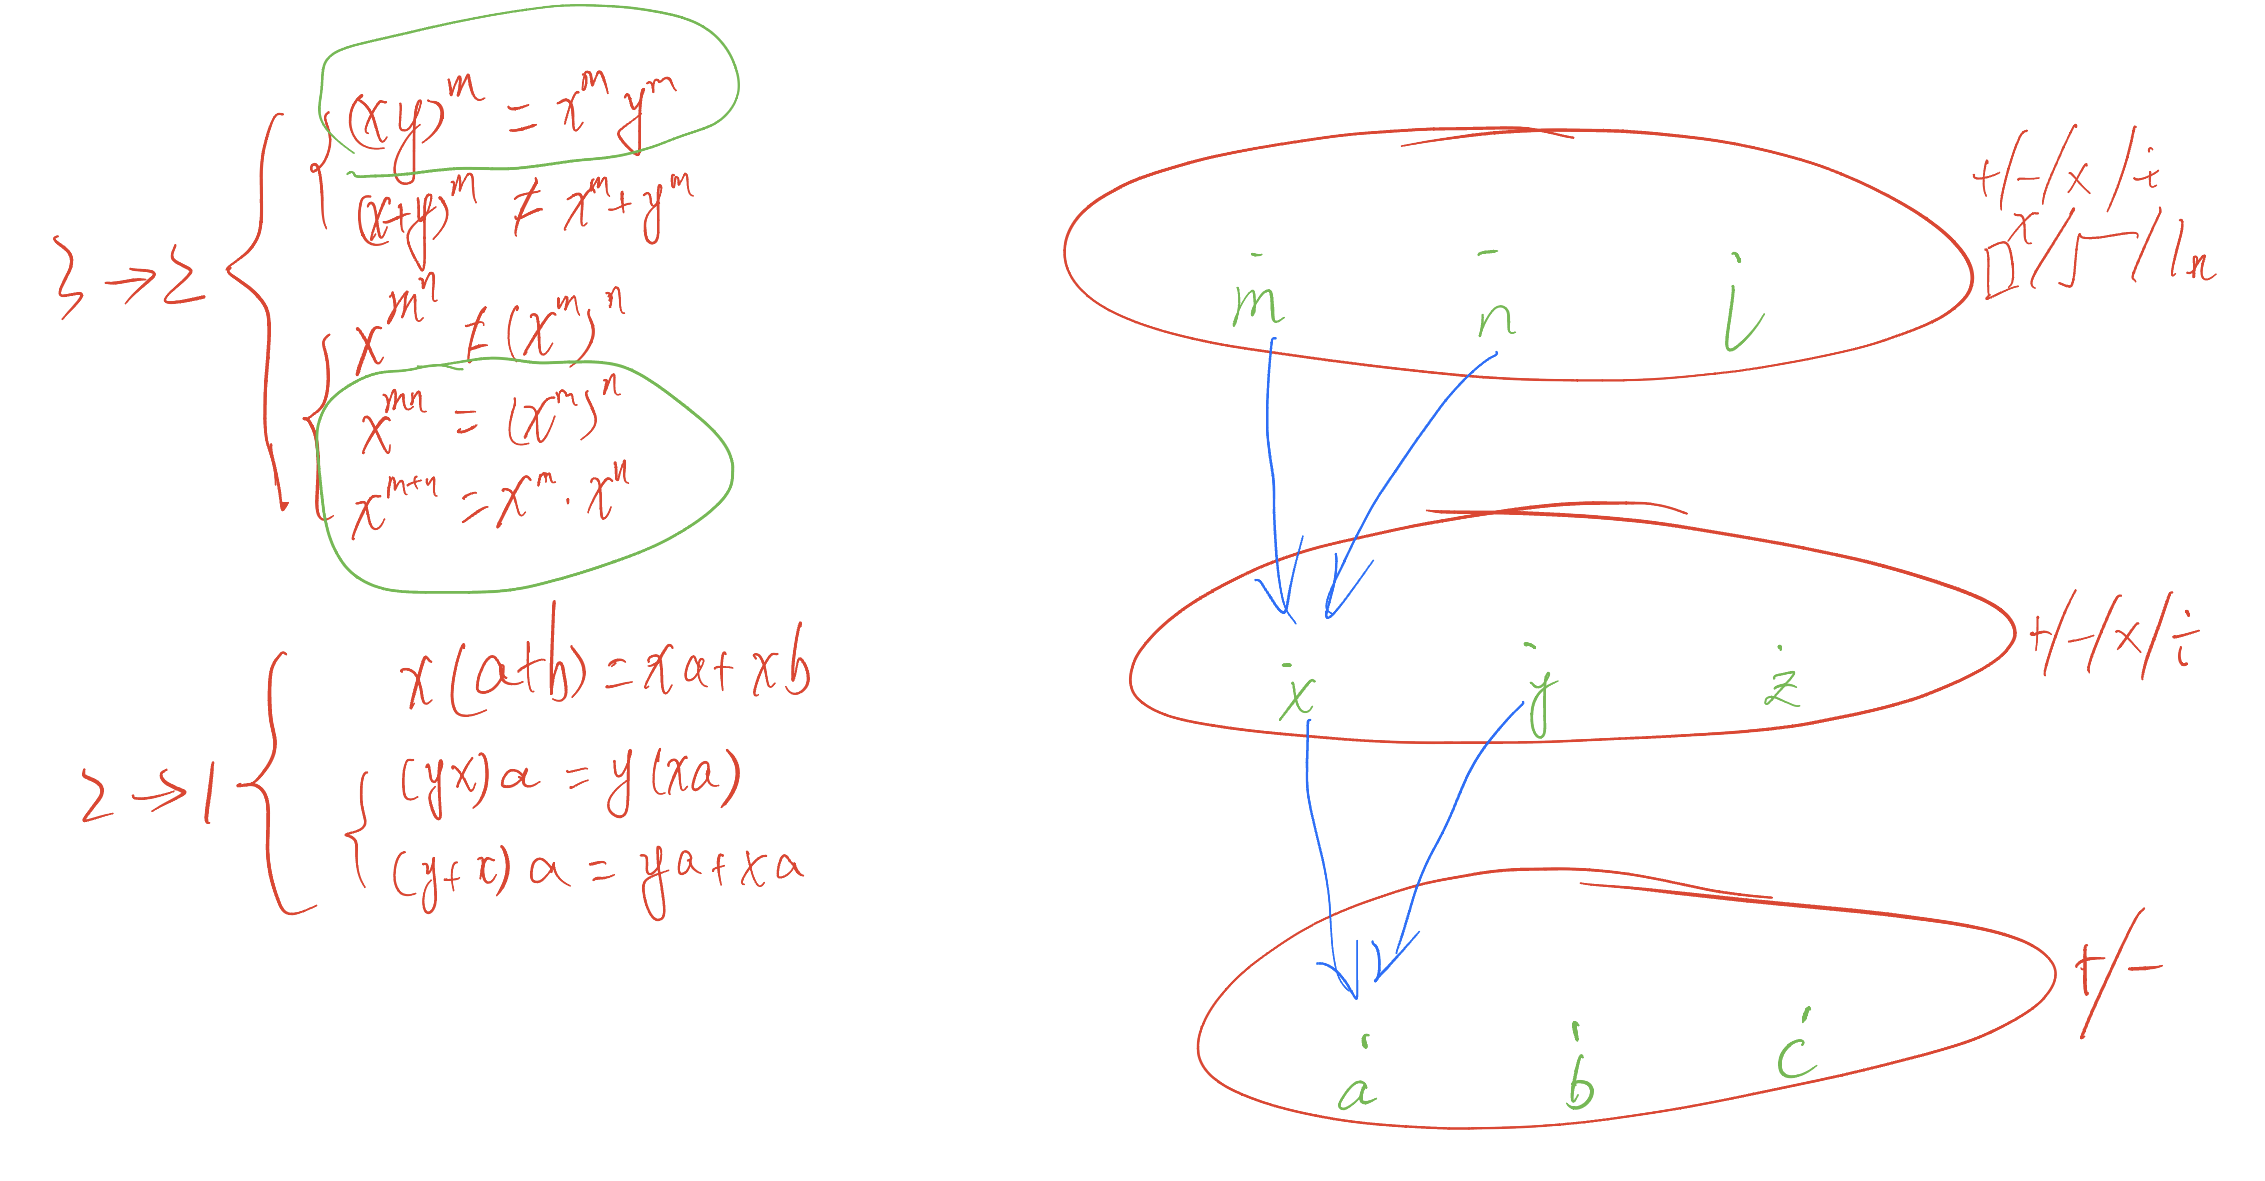
\includegraphics[width=0.86\textwidth]{images/operations.png}


\newpage

\section{课程脚本}
\begin{tabularx}{0.99\textwidth}{ 
  | >{\centering\arraybackslash}X 
  | >{\centering\arraybackslash}X | }
 \hline
 \textbf{脚本}  & \textbf{动画} \\
 \hline
\end{tabularx}


\begin{tabularx}{0.928\textwidth}{ 
  | >{\raggedright\arraybackslash}X 
  | >{\raggedright\arraybackslash}X | }
加减乘除是我们再熟悉不过的数学运算,甚至在不少人的认识里,加减乘除是数学的代名词。这个朴素的印象来源于我们在小学得到的数学教育,这个视频我们将会揭示出加减乘除

 
& 


 
\\
\hline
\end{tabularx}
 










\end{CJK*}

\bigskip  %% Just some white space




\end{document}